\subsection{Dinámica}
    \noindent A partir de la expresión (\ref{eqn:DL_final}) considerando el \emph{principio de D'Alamabert-Lagrange} para sistemas con efectos de
    disipación y potencial gravitacional conservativo. Puede construirse el modelo dinámico del sistema:
    \begin{equation}
        \label{eqn:modelo_dinamico}
        \boldsymbol{\ddot{q}} =H(\boldsymbol{q})^{-1} \left \{ \boldsymbol{\boldsymbol{\tau}} - C(\boldsymbol{q}, \boldsymbol{\dot{q}}) \boldsymbol{\dot{q}}
        - D(\boldsymbol{q}, \boldsymbol{\dot{q}}) - \boldsymbol{g}(\boldsymbol{q}) \right \}
    \end{equation}
    donde el vector de torques $\boldsymbol{\tau}$ representa la entrada del sistema y $\boldsymbol{\ddot{q}}$ la salida del mismo. 
    
    Para realizar la simulación, es necesario obtener de manera simbólica en función de $(\boldsymbol{q}, \boldsymbol{\dot{q}})$ la estructura
    de cada término en (\ref{eqn:modelo_dinamico}). 

    \subsubsection{Matriz de inercia simbólica}
    \noindent Para obtener la matriz de inercia en términos de las coordenadas generalizadas, se optó por construir la función del Anexo \ref{cd:inercia} con base a la expresión
    (\ref{eqn:inertia_matrix}). De este modo, al integrar dos veces la aceleración $\boldsymbol{\ddot{q}}$ podrá utilizarse para evaluar $H(\boldsymbol{q})$
    mediante el uso de \emph{Simulink}. 

    Mientras que los valores de los jacobianos geométricos para cada centro de masa está dado por (\ref{eq:Jv}) y (\ref{eq:Jw}), mientras que los tensores de inercia (con valores
    en el Anexo \ref{Tensores}) de cada eslabón fueron obtenidos mediante el análisis de propiedades físicas de \emph{SolidWorks}.

    \subsubsection{Vector de Coriolis simbólico}
    \noindent Una vez obtenida la matriz de inercia de manera simbólica, puede procederse con el cálculo del vector de Coriolis $C(\boldsymbol{q}, \boldsymbol{\dot{q}})\boldsymbol{\dot{q}}$ mediante
    los símbolos de Christoffel expuestos en (\ref{eqn:christoffel}) tal como se presenta en la función de \emph{MATLAB} del Anexo \ref{cd:coriolis}. 

    \subsubsection{Vector de disipación simbólico}
    \noindent Mientras que $D(\boldsymbol{q}, \boldsymbol{\dot{q}})$ está basada en la expresión (\ref{eqn:disipacion_simple}) con coeficientes de fricción
    viscosa iguales para cada articulación; suponiendo así, que la fricción dado el rozamiento entre componentes mecánicos y el motor es la misma para cada articulación. 

    Cabe destacar que $b$ es un parámetro que el usuario podrá modificar en un intérvalo de $0$ a $0.1$ $[\frac{Ns}{m}]$, con el fin de tener un análisis más amplio sobre
    el robot. Por lo que al tener un valor de $b=0$, se asume que el sistema no perderá energía dados los efectos de disipación y por ende, será un sistema conservativo. 

    \subsubsection{Vector de gravedad simbólico}
    \noindent Como último componente del modelo dinámico, $\boldsymbol{g}(\boldsymbol{q})$ fue obtenido a partir de la expresión (\ref{eqn:vector_gravedad}). Donde
    \begin{equation}
        \label{eqn:g_0}
         \boldsymbol{g}_0 = \begin{bmatrix} 0 & 0 & -9.81 \end{bmatrix}^T
    \end{equation}

    está en coordenas inerciales con unidades en $[\frac{m}{s^2}]$. Su construcción se presenta en el Anexo \ref{cd:gravedad}.

    \subsubsection{Simulador Dinámico}
    \noindent Considerando que \emph{Simulink} funciona mediante bloques, cada una de los términos requeridos por (\ref{eqn:modelo_dinamico}) pueden ser exportados mediante la
    función \emph{matlabFunctionBlock} \cite{matlabFunctionBlock}. Por lo que al implementarse, se obtiene el diagrama de bloques de la Figura \ref{fig:diagrama_bloques}.
    \begin{figure}[H]
        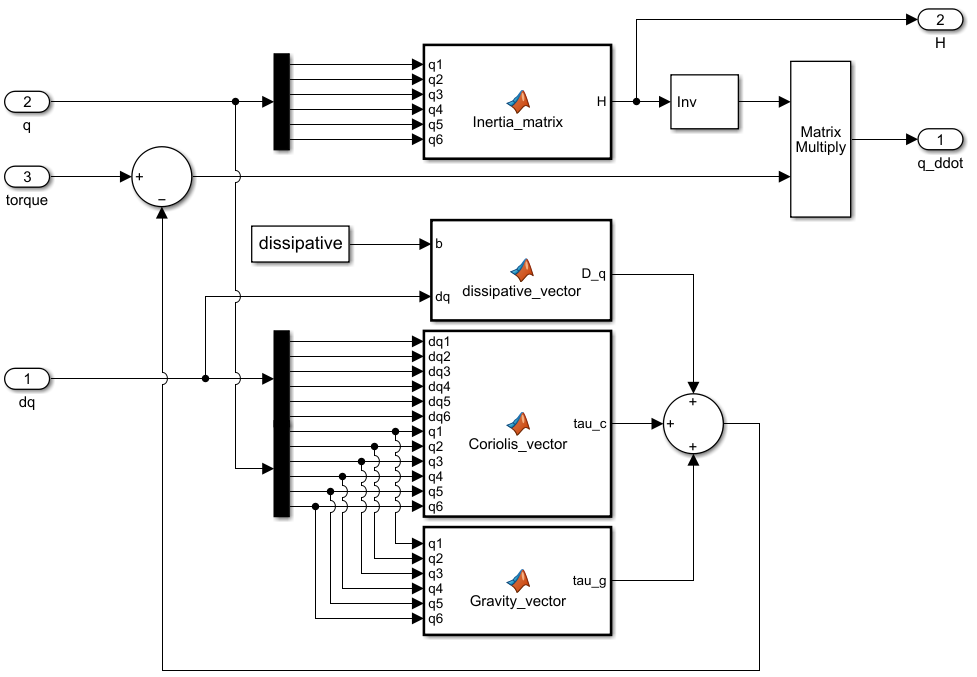
\includegraphics[scale = 0.38]{diagrama_bloques.png}
        \centering
        \caption{Diagrama de bloques del modelo dinámico}
        \label{fig:diagrama_bloques}
    \end{figure}
    Donde \emph{dissipative} representa al factor de disipación $b$ indicado por el usuario, \emph{torque} es equivalente a $\boldsymbol{\tau}$; mientras que 
    $dq$ y $q$ indican $\boldsymbol{\dot{q}}$ y $\boldsymbol{q}$ respectivamente. 
    
    Como salidas, se define la matriz de inercia $H(\boldsymbol{q})$ evaluada y la aceleración $\boldsymbol{\ddot{q}}$.
    \begin{figure}[H]
        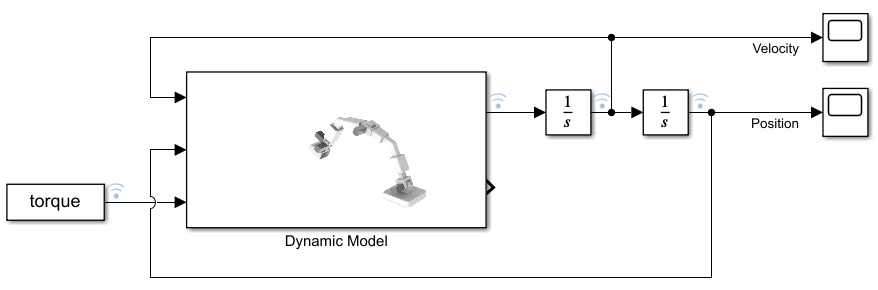
\includegraphics[scale = 0.39]{simulador1.png}
        \centering
        \caption{Diagrama de bloques de la planta}
        \label{fig:planta}
    \end{figure}
    
    \subsubsection{Solucionador}
    %\textbf{Pendiente para revisar el caso conservativo}
    Considerando que para la simulación es necesario integrar $\boldsymbol{\ddot{q}}$ para obtener las variables de estado,
    es requerido el uso de un solucionador. Para el simulador, se optó por el $ode15s$, un solucionador de paso variable y orden variable (\emph{VSVO}), basado en las fórmulas de diferenciación numérica
    (\emph{NDF}) de los órdenes 1 a 5, pero que a su vez, puede utilizar las fórmulas de diferenciación inversa (\emph{BDF}) que suelen ser menos eficientes \cite{ode15s}. 
    
    Al igual que $ode113$, $ode15s$ es un solucionador de paso variable destinado a resolver ecuaciones diferenciales rígidas y ecuaciones algebraicas diferenciales (\emph{DAE}). 
    Con respecto al concepto de los ODE rígidos, se explica en \cite{ODEs} que hace referencia a aquellos sistemas que presentan tramos de variación rápida en ciertas secciones de
    la función, mientras que hay otras en las que el cambio es lento en comparación a otras regiones, lo cual conlleva a tamaños de paso extremadamente pequeños, ocasionando que
    integradores de paso fijo como el $ode45$ fallen al converger, o bien, que tomen mucho tiempo en lograrlo.

    Respecto a los parámetros de los integradores, se consideró las condiciones iniciales del sistema en \emph{casa}. Es decir, 
    \begin{equation*}
        \label{eqn:init_q}
        \boldsymbol{q}(0) = 0
    \end{equation*}
    \begin{equation*}
        \label{eqn:init_dq}
        \boldsymbol{\dot{q}}(0) = 0
    \end{equation*}

    \subsubsection{Energía Potencial}
    \noindent Considerando que el modelo dinámico está obtenido con base a un análisis energético, es conveniente conocer como se comporta la energía cinética, potencial y mecánica del 
    sistema para la validación del modelo, así como para la selección de técnicas de control como trabajo a futuro.
    
    Por lo tanto, se realizó la implementación de la expresión
    (\ref{eqn:energia_potencial}) como se presenta en el Anexo \ref{cd:energia_potencial}. Sin embargo, para las gráficas se consideró el ajuste del \emph{datum} con el fin de
    evitar valores negativos en la energía potencial tal como se presenta en (\ref{eqn:energia_potencial_offset}), donde $U_0$ corresponde al valor mínimo de $U$ durante el
    tiempo de simulación. 

    \subsubsection{Energía Cinética y Mecánica}
    \noindent Para el cálculo de la energía cinética no fue necesaria la construcción de una función, dado que la matriz de inercia ya se encuentra evaluada durante la simulación como
    se presenta en la Figura \ref{fig:diagrama_bloques}. Por lo que únicamente se aplicó (\ref{eqn:kinetic_energy}) para su cálculo. 

    Mientras que para la energía mecánica se considero la expresión (\ref{eqn:energia_mecanica}).